\documentclass{article}
\usepackage{paper}

\setpapertitle{Mixture of Experts using Discrete VAE}

\addauthor{Abhisek Panda}{150026}
\addauthor{Aakarsh Gajbhiye}{150000}

\begin{document}
\makeheader

\abstract{
	A lot of data in the real world exists in arbitrarily shaped clusters. Applying regression/classification models to such data can be pointless if the complexities of the hypothesis class of these models is low. Mixture of experts try to solve this problem by using a different expert/learner for each cluster, therefore creating a prediction using not one, but a mixture of learnt experts. We propose a superior gating function for these mixture of experts using Variational Autoencoders designed to perform as gating functions.
}

\begin{psection}{Introduction}

	Humans can perceive cluster patterns in data even with arbitrarily sized and shaped clusters. The same cannot be said for most machine learning models. In fact, most Mixture of Experts (ME) models are built assuming the underlying clusters of the data to be simple gaussians. This problem can, however, be alleviated by using latent variable models.

	Latent variable models essentially decode the inherent properties of the data. In the latent space, since the complexities of the data are unravelled, the clusters are simple enough to be modelled properly as gaussians. Such clustering still allows arbitrary cluster shapes in the original space.

	We use the same idea, and construct a generative model based on Variational Autoencoders(VAE) to find apt latent variables. Using this, we cluster the data, and form a simple gating function based on a Feed Forward Neural Network. The model is explained in detail in Section 3. We observe interesting results, with our model outperforming naive gating functions by a huge margin. These experiments are recorded in section 4.

\end{psection}

\begin{psection}{Background}

	\begin{psubsection}{(Generative) Latent Variable Models}
		Latent variables are variables that are not directly observed but are rather inferred from other variables that are observed \cite{wiki-latent-vars}. Suppose we have a task of creating digits (such as in MNIST), it would help to know which digit (0-9) we wish to create, what should be the width of the digit, at what angle should the digit be tilted. Such decisions can be informally called as latent variables, as these decisions, in a generative story, help us to create the digits, and in an inference story, help us understand the inherent properties of the digits.

		Such a model where we actually generate data similar to the provided training data are known as generative models. A formal description of a generative model with latent variables is described below.

		Say, we have a vector of latent variables $\vz$ in a lower-dimensional space $\cZ$, which we can easily sample according to some probability density function (pdf) $\prob{\vz}$  defined over $\cZ$. Moreover, we also have a family of deterministic functions $f(\vz; \vtheta)$, parameterized by $\vtheta$ in some space $\vTheta$, such that $f : \cZ \times \vTheta \rightarrow \cX$, where $\cX$ denotes the original data space. Our objective, therefore, is to find the correct set of parameters $\vtheta$ so that the construction of the generated data is closest to the real data. More formally, we want to find a function $f$, such that the quantity
		\begin{align*}
			\prob{\vx} = \int_\vz \prob{\vx \pipe \vz, \vtheta} \cdot \prob{\vz} \id\vz
		\end{align*}
		is maximized. For example, the probability $\prob{\vx \pipe \vz, \vtheta}$ can be formulated as $\ND{\vx \pipe f(\vz; \vtheta), \sigma^2 \vI}$ in case $\cX \in \bR $. The intuition behind this framework—called \et{maximum likelihood} is that if the model is likely to produce training set samples, then it is also likely to produce similar samples, and unlikely to produce dissimilar ones.

		Each generative model is defined by a generative story which allows us to visually interpret the interdependence of variables, more particularly dependence of observed variables on the defined latent variables.

		In most cases, the posterior of the latent variables given a data point ($\prob{\vz \pipe \vz}$) is in intractable form. In such cases, these models are trained using methods such as Monte Carlo Markov Chain(MCMC) or Variational Inference. Popular choices of generative models include variants of the vanilla Variational Autoencoder \citep{vae}. The reasons for the same are that the VAE architecture allows us to perform amortized inference (details in the next section). We take a deeper look at latent variable models in the following sections.
	\end{psubsection}

	\begin{psubsection}{Gaussian Mixture Models}
		A simple Latent Variable Model is the Gaussian Mixture Model (GMM). GMMs are useful for modeling data that come from one of several groups, with each group being modeled by a Gaussian distribution. It is used for data clustering and density estimation. The model assumes data generated for a mixture of $K$ gaussians with mixing proportion $\vpi = \brac{\pi_1 \dots \pi_K}$. Intuitively, each $\pi_k \in (0,1)$ represents the fraction of data contributed by the k\tth Gaussian.

		In this model, we define the latent variable to be the cluster assignment of each data point, \ie $z$ represents the index of the cluster the corresponding data point belongs to with a categorical/discrete prior. Therefore, the mixing proportion can now be formally defined as the weights of the categorical distribution representing the prior of the latent variable $z$. Hence, we can write
		\begin{align*}
			\prob{z = k \pipe \vpi}			&\eq \pi_k \\
			\implies \prob{z \pipe \vpi}	&\eq \prod_{k = 1}^K \para{\pi_k}^{\is{z = k}}
		\end{align*}

		Since we now have a cluster assignment, the next step is to define the probability distribution we use for sampling each data point. As pointed out earlier, this probability distribution is given by a gaussian.
		\begin{align*}
			\prob{\vx \pipe z = k} \eq \ND{\vx \pipe \vmu_k, \vSigma_k^{-1}}
		\end{align*}

		Since doing straight-forward MLE is not possible for this model (due to the presence of latent-variables), we estimate the parameters $\set{\vmu_k, \Sigma_k}_{k = 1}^K$ using Expectation Maximization(EM) Algorithm, which is a popular strategy for simple latent-variable models.

		The problem with GMM is the assumed Gaussian structures for each cluster. As pointed out earlier, this limits the power of GMM therefore not allowing arbitrary clustered data to be modeled using such models. We therefore need to explore other latent variable models with higher reprentational/expressive power. One such model is the Variational Deep Embeddings (VaDE) Model \citep{vade}, based on the Variational Autoencoder architecture. We discuss this model in the next section.
	\end{psubsection}

	\begin{psubsection}{Variational Autoencoders}
		Variational Autoencoders were initially proposed by \cite{vae}. The key idea behind VAEs is that any distribution in $D$ dimensions can be generated by taking a set of $D$ variables that are normally distributed and mapping them through a sufficiently complicated function \citep{vae-tut}. Hence, provided powerful function approximators, we can simply learn a function which maps independent, normally distributed variables to the latent variables needed for our model, and these latent variables are then used to model the observations $\vX$, or rather the data distribution $\cD$ not known to us, from which the observations are assumed to be sampled.

		The task, therfore, is to find a strong non-linear mapping to approximate the latent variables needed to model the data distribution $\cD$. This mapping, in VAEs, is modelled using a neural network, and the mapping from these latent variables to the observations is through a distribution (generally exponential family) depending on the observed space $\cX$. For example, if $\cX \in \bR$, then the estimated probability distribution for $\vx \sim \cD$ can be given as
		\begin{align*}
			\prob{\vx \pipe \vz} \eq \ND{\vx \pipe f(\vz; \vtheta), \sigma^2 \vI}
		\end{align*}
		for some non-linear mapping $f: \bR \ra \bR$ (in this case) modelled using a neural network.

		The objective now is to compute the posterior over $\vz$ given the observation $\vx$. This would allow us to model the predictive posterior using samples of $\vz$ from this posterior. Since the posterior $\prob{\vz \pipe \cD}$ is intractable, we approximate it using a proposal distribution $\cQ(\vz \pipe \vx, \vphi)$. We use the standard Black Box Variational Inference strategy to estimate the posterior, by maximizing the ELBO bound using descent methods, which is given as
		\begin{align*}
			\cL(\vx; \cQ) &\eq \log{\prob{\vx}} - \text{KL}\brac{\cQ(\vz; \vphi)\ ||\ \prob{\vz \pipe \vx}} \\
			&\eq \E[\vz \sim \cQ(\vz \spipe \vx, \vpi)]{\log{\frac{\prob{\vx, \vz}}{\cQ\para{\vz \pipe \vx, \vphi}}}}
		\end{align*}
		Typically, the prior over the latent variables $\vz$ is assumed to be a multivariate normal distribution with mean $\vzero$ and variance matrix $\vI$.

		This structure is similar to that of a standard autoencoder, where the network which maps the inputs to the parameters of the proposal is the encoder and the network mapping the sampled $\vz$'s to the parameters of the conditional likelihood distribution is the decoder.

		One major problem with Variational Inference is that it models the parameters of each latent variable independently, and therefore we need an iterative procedure to model the proposal with respect to each variable. That is, if we want to add a new data point, we need to remodel the proposal in order to compute the pdf of the new latent variable. VAE tackles this problem by assuming that the latent variable is dependent on the input, and the mapping from the input to the parameters of the proposal distribution is modeled using a neural network. This, essentially, is the idea of amortized inference.

		Since looking at the ELBO, one can say we wish to minimize the KL Divergence between the proposal and the prior for $\vz$ which is a standard Normal distribution, we can assume the proposal to be of the form \ $\ND{\vz \pipe \vmu(\vx; \vphi), {\vsigma}^2(\vx; \phi) \vI}$. The negative ELBO is then considered as our loss, and the parameters (or weights) of the Neural Networks are inferred.

		However, since we are assuming the variables $\vz$ to be sampled from the proposal, we cannot apply back propogation across the decoder and the encoder networks. This is handled using the reparameterization trick, where we write $\vz = \vepsilon \cdot {\vsigma}^2(\vx; \vphi) + \vmu(\vx; \vphi)$. This allows us to input the reparametrized latent variables $\vepsilon$, and therefore facilitate backpropogation through the stochastic nodes. The working of a standard VAE is visuallized in figure \ref{fig:VAE} \footnote{Image taken from \cite{vae-tut}}.

		\begin{figure}
			\centering
			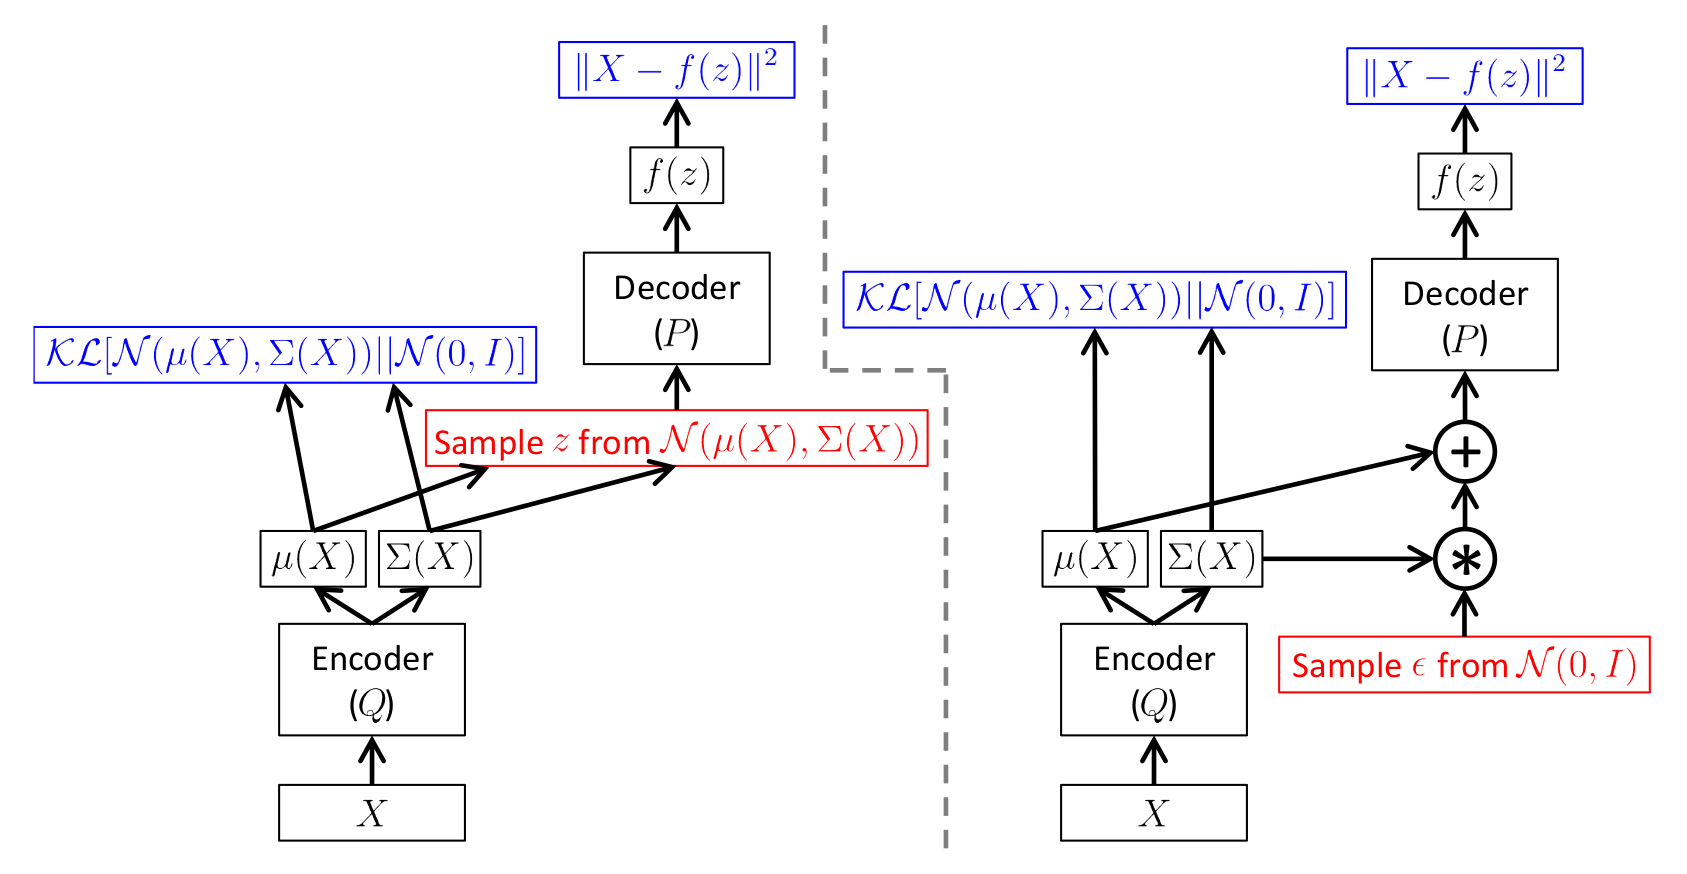
\includegraphics[width=0.9\textwidth]{includes/vae.png}
			\caption{Without (left) and with (right) the reparametrization trick}
			\label{fig:VAE}
		\end{figure}

	\end{psubsection}

\end{psection}

\begin{psection}{Variational Deep Embeddings}

	Variational Deep Embedding (VaDE) was proposed by \cite{vade}. It is a simplistic model than the previous models discussed, and greatly simplifies the generic generative story by assuming a uniform prior on the cluster means, variances, and misture proportions. Also, it assumes a uniform prior on the model parameters $\vtheta$.

	\begin{figure}[h]
		\centering
		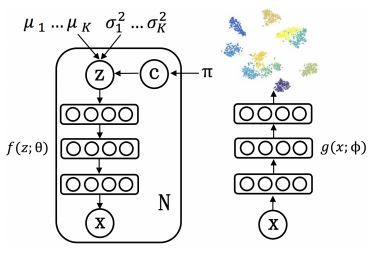
\includegraphics[height=150px]{includes/vade.jpg}
		\caption{Plate notation for VaDE (left) and an encoder network $g(\vx; \phi) (right)$}
		\label{fig:my_label}
	\end{figure}

	Depending on whether the observations $\vx$ is binary or real-valued we compute $\mu_x = f(\vz, \vtheta)$ and choose a sample $\vx \sim Ber(\mu_x)$ or compute $[\mu_x;\log\sigma^2_x] = f(\vz,\vtheta)$ and choose a sample $\vx \sim \mathcal{N}(\mu_x,\sigma^2_x\vI)$. From the generative story, the joint probability can be written as
	\begin{align*}
		\prob{\vx, \vz, c} \eq \prob{\vx \pipe \vz, \vtheta} \prob{\vz \pipe c} \prob{c}
	\end{align*}

	An instance of VaDE is tuned to maximize the likelihood of the given data points. Given the generative process described above we have
	\begin{align*}
		\logp{\prob{\vx}} &\eq \log{\int_\vz \sum_c \prob{\vx, \vz, c} \id \vz} \\
		&\qge \E[\cQ(\vz, c \spipe x)]{\logp{\frac{\prob{\vx, \vz, c}}{\cQ(\vz, c \pipe \vx)}}} \eq \cL_{\text{ELBO}}
	\end{align*}
	where $\cQ(\vz, c \pipe \vx)$ is the proposal distribution.

	Mean field is assumed on the proposal distribution, giving:
	\begin{align*}
		\cQ(\vz, c \pipe \vx) &\eq \cQ(\vz \pipe \vx) \cQ(c \pipe \vx)
	\end{align*}

	Similar to VAE, the distribution $\cQ(\vz \pipe \vx)$ is modelled using a neural network $g$ as follows
	\begin{align*}
		\tilde{\vmu}, \logp{\tilde{\vsigma}^2} &\eq g(\vx, \vphi) \\
		\cQ(\vz \pipe \vx) &\eq \ND{\vz \pipe \tilde{\vmu}, \tilde{\vsigma}^2 \vI}.
	\end{align*}

	Further, a decoder model is added giving the following:
	\begin{align*}
		\prob{\vx \pipe \vz} &\eq \prob{\vx \pipe f(\vz, \vtheta)}
	\end{align*}

	The authors use an interesting approach to ``approximating'' the proposal distribution $\cQ(c \pipe \vx)$, which although looks absurd, in practice works surprisingly well. First, one can realize, the ELBO can be re-written in the following manner,
	\begin{align*}
		\cL_{\text{ELBO}} &\eq 	\E[\cQ(\vz, c \spipe \vx)]{\logp{\frac{\prob{\vx, \vz, c}}{\cQ(\vz, c \pipe \vx)}}} \\
		&\eq					\int_{\vz} \sum_{c} \cQ(c \pipe \vx) \cQ(\vz \pipe \vx) \set{\logp{\frac{\prob{\vx \pipe \vz} \prob{\vz}}{\cQ(\vz \pipe \vx)}} + \logp{\frac{\prob{c \pipe \vz}}{\cQ(c \pipe \vx)}}} \\
		&\eq \int_{\vz} \cQ(\vz \pipe \vx) \logp{\frac{\prob{\vx \pipe \vz} \prob{\vz}}{\cQ(\vz \pipe \vx)}} \id \vz - \int_{\vz} \cQ(\vz \pipe \vx) \kld{\cQ(c \pipe \vx)}{\prob{c \pipe \vz}} \id \vz
	\end{align*}

	In order to maximize the above ELBO, it seems we need to minimize the average KL Divergence over the latent variables, when sampled using the posterior. \et{Jiang et al.} approximated this simply using only one sample of $\vz$ and therefore, we can write 
	\begin{align*}
		\cQ(c \pipe \vx) \eq \prob{c \pipe \vz = \hat{\vz}} \eq \frac{\prob{c} \prob{\vz = \hat{\vz} \pipe c}}{\sum_{c' = 1}^{K} \prob{c'} \prob{\vz = \hat{\vz} \pipe c'}}
	\end{align*}
	where $\hat{\vz}$ is a sample from the posterior proposal $\cQ(\vz \pipe \vx)$.

	Given the simplicity of the model, we performed some experiments on it. We implemented the complete model on Tensorflow from scratch, and performed experiments on a couple of datasets. This is discussed in detail in the following section.
\end{psection}

\begin{psection}{Mixture of Experts (ME)}
	Just like GMM, a mixture of experts model splits the data into soft clusters, and for each cluster, we have an expert which predicts the target labels for each mixture. Therefore, we need to define a \et{gating function}, which defines the mixing proportions for each data point. Suppose we denote the mixture assignment using a latent variable $c$, then we have a probability density/mass function $\prob{\vy \pipe \vx, c}$. Mostly this probability is defined using a pdf function belonging to the class of exponential distributions. For example, if the space of the target label $\cY = \set{0, 1}$, then we can define $\prob{\vy \pipe \vx, c}$ to be a Bernoulli distribution.

	We still need to define a mixing proportion. Since our ultimate goal is to model $\prob{\vy \pipe \vx}$, we write
	\begin{align*}
		\prob{\vy \pipe \vx} &\eq \sum_{k = 1}^K \prob{\vy, c = k \pipe \vx} \\
		&\eq \sum_{k = 1}^K \prob{c \pipe \vx} \cdot \prob{\vy \pipe c = k, \vx}
	\end{align*}

	Looking at the above equation, we can say setting $\prob{c \pipe \vx}$ to be the mixing proportion as a natural choice. The most common choice for modelling this probability mass function is using a softmax distribution as follows -
	\begin{align*}
		\prob{c = k \pipe \vx} \eq \frac{\texp{b_k + \dotp{\vw_k}{\vx}}}{\sum_{k' = 1}^K \texp{b_{k'} + \dotp{\vw_{k'}}{\vx}}}
	\end{align*}
	where K is the number of experts.

	We usually represent $\prob{c = k \pipe \vx}$ using the function $g_k(\vx, \vTheta_g)$. To sum up ME models, $g_k(\vx, \vTheta_g)$ is essentially the gate's rating for the k\tth expert given $\vx$ and $\prob{\vy \pipe \vx, c, \vTheta_e}$ is the probability of the k\tth expert generating $\vy$ given $\vx$. For brevity, we denote this as $p_i(\vy)$.

	In general, the ME training algorithm maximizes the log-likelihood $\prob{\vy \pipe \vx}$ to learn the parameters of the expert and the gate. During the training ME, the gate and the experts gets decoupled, therefore the model attains a modular structure. This property is exploited in order to extend ME models to hierarchical mixture of experts (HME). A standard ME model is graphically represented in figure \ref{fig:me} \footnote{Image taken from \cite{me-image}}.

	\begin{figure}[htpb]
		\centering
		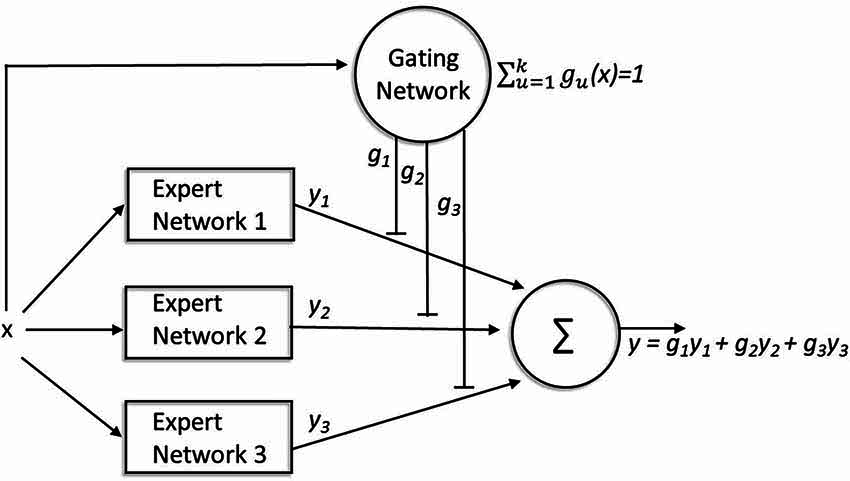
\includegraphics[width=0.7\textwidth]{includes/me.png}
		\caption{Graphical representaion of a standard Mixture of Experts model}
		\label{fig:me}
	\end{figure}

	\begin{psubsection}{ME Regression Model}

		Let $\vTheta_e = \set{\sW_k, \Gamma_k}_{k = 1}^{K}$ denote the parameters of the experts. As mentioned earlier, in the original ME regression model, the experts follow the gaussian model -
		\begin{align*}
			\prob{\vy \pipe \vx, c = k} \eq \ND{\vy \pipe \hat{\vy}(\vx, \sW_k), \Gamma_k}
		\end{align*}
		where $\vy \in \bR^\sM$. The term $\hat{\vy}(\vx, \sW)$ is defined as $\hat{\vy}(\vx, \sW) = \sW \vx$. We can also add a bias term to $\sW \vx$.

		At test time, in order to make a prediction, the expectation of $\vy$ with respect to the pdf $\prob{\vy \pipe \vx,\vTheta}$ is used as the output of the architecture. This is, therefore, given by
		\begin{align*}
			\hat{\vy} = \sum_{k = 1}^K g_k(\vx, \vTheta_g) \cdot \hat{\vy}(\vx, \sW)
		\end{align*}
	\end{psubsection}

	\begin{psubsection}{ME Classification Model}
		In this case, the probability of $\vy$ is given by a categorical/discrete distribution. In the one hot representation, the desired output $\vy$ is of length L and $y_l$ = 1 if $\vx$ belongs to class $l$ and 0 otherwise. Also, expert $k$ has parameters $\set{\vw_{imk}}_{k = 1}^K$, corresponding to the parameters of each class. The probability given by each expert is therefore written as
		\begin{align*}
			\prob{\vy \pipe \vx, c = k} &\eq \prod_{l = 1}^L \hat{\vy_l}(\vx, b_k, \vw_k)^{\is{y_l = 1}} \\
			\hat{\vy_l} &\eq \frac{\texp{\dotp{\vw_{ik}}{\vx}}}{\sum_{l' = 1}^L \texp{\dotp{\vw_k}{\vx}}}
		\end{align*}

		The prediction is done in the same way as was shown for the ME Regression Model.

	\end{psubsection}

	Although the paradigm of Mixture of Experts is very generic, not many methods exist for the same. The fundamental problems are the difficulties of inference, along with non-compatibility with automatic differentiation libraries for the existing inference methods. We try to remedy this problem by proposing a novel Mixture of Experts model based on Variational Autoencoders. In the next section, we show a way to extend the VaDE model for use as a gating function for ME models, and point out some difficulties in doing the same. Following that, we propose a novel gating function based on Discrete Latent Variables in Variational Autoencoders, and later show that it outperforms other naive gating functions.
\end{psection}

\begin{psection}{VaDE with Mixture of Experts}
% Add Theory on VaDE as gating function ( Loss + Inference method)
% Add problems in this (test time inaccuracy + slow inference <- due to inaccurate estimation of p(c | x, y) (same problem with original vade))
	The VaDE model originally described in \cite{vade} is used to learn cluster assignments and also work as a generative model. For using VaDE in classification/regression tasks, the original theory can be extended in a straight-forward manner by maximizing the log of joint probability for $\vX$ \& $\vY$.
	\begin{align*}
		\logp{\prob{\vx, \vy}} &\eq \log{\int_\vz \sum_c\prob{\vx, \vy, \vz, c}} \\
		&\qge \E[\cQ(\vz, c \spipe \vx, \vy)]{\logp{\frac{\prob{\vx, \vz, c}}{\cQ(\vz, c \pipe \vx, \vy)}}} \eq \cL_{\text{ELBO}}
	\end{align*}
\end{psection}

\begin{psection}{Discrete Variational Mixture of Experts}

	As pointed out in the previous section, VaDE suffers from two prime problems, slow inference and slow and inaccurate predictions. We try to design a gating function keeping these two problems in mind.

\end{psection}

\begin{psection}{Experiments}

	\begin{psubsection}{VAE Training}

	% Breifly highlight differences between the model in terms of learning cluster assignments
	% VaDE vs Our model reconstruction + TSNE + sampling plots

	\end{psubsection}

	\begin{psubsection}{ME Results}

	% Results of our model vs DMOE vs (if possible) VaDE ME

	\end{psubsection}

\end{psection}

\begin{psection}{Related Work}

\end{psection}


\begin{psection}{Conclusion}

\end{psection}

\bibliographystyle{plainnat}
\bibliography{main}

\end{document}

